% !TEX TS-program = xelatex
% !TEX encoding = UTF-8 Unicode
% !Mode:: "TeX:UTF-8"
\documentclass{resume}
\usepackage{graphicx}
\usepackage{tabu}
\usepackage{multirow}
\usepackage{progressbar}

\usepackage{zh_CN-Adobefonts_external} % Simplified Chinese Support using external fonts (./fonts/zh_CN-Adobe/)
% \usepackage{NotoSansSC_external}
% \usepackage{NotoSerifCJKsc_external}
% \usepackage{zh_CN-Adobefonts_internal} % Simplified Chinese Support using system fonts
\usepackage{linespacing_fix} % disable extra space before next section
\usepackage{cite}
\usepackage{graphicx} % 确保你已经加载了 graphicx 包（用于插入图片）
\begin{document}
\pagenumbering{gobble} % suppress displaying page number

\name{邹杰}

\normalsize
\begin{tabu}{ l c r }  % 左对齐、居中、右对齐
  \textbf{ } & & 
 \multirow{3}{1in}{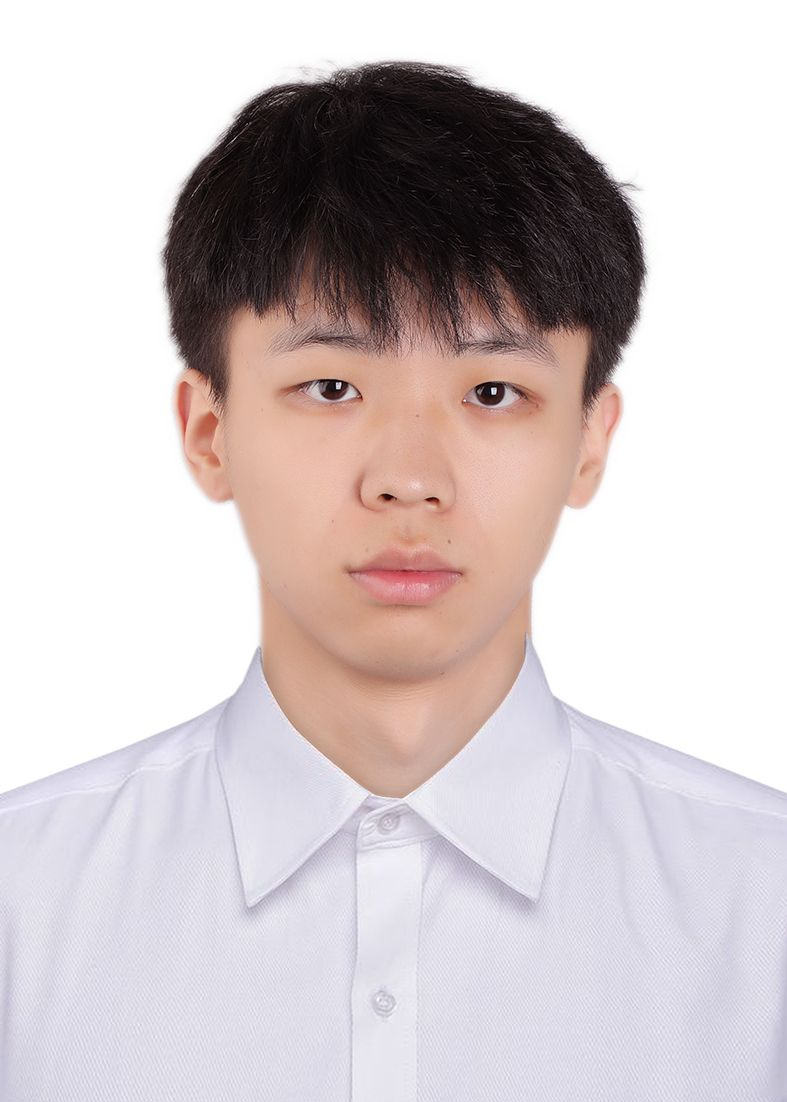
\includegraphics[width=0.57in]{picture}} \\
  
   \phantom{11111111111111111111111111111111111111111111111111111111111111111111111111}& & \\
  
  \email{1991645643@qq.com} \textperiodcentered\ 
  \phone{(+86) 18684144634}& & \\
\end{tabu}

 
\section{\faGraduationCap\  教育背景}
\datedsubsection{\textbf{华中科技大学}, 武汉}{2023 -- 至今}
\small\textit{在读硕士研究生}\ 计算机科学与技术学院, 计算机技术 
\datedsubsection{\textbf{南京邮电大学}, 南京}{2019 -- 2023}
\small\textit{学士}\ 软件学院，软件工程

\section{\faCogs\ 专业技能}
% increase linespacing [parsep=0.5ex]
\begin{itemize}[parsep=0.5ex]
  \item 熟练C/C++，C++的封装继承多态，使用C的指针应用及内存管理，STL常用容器，C++11常用特性
  \item 熟练掌握数据结构和算法、计算机网络、操作系统等计算机基础知识
  \item 熟悉Linux下开发环境，了解网络编程，IO多路复用，epoll等
  % \item 熟悉OSI五层网络模型，熟悉TCP/IP,UDP,HTTP/HTTPS,DNS等网络协议，熟悉TCP三次握手，四次挥手，流量控制，拥塞控制等手段
  \item 熟练使用 MySQL，熟悉 MySQL 索引、事务、存储引擎、锁机制
  % \item 熟悉使用Git，vscode等工具。
  \item 熟悉常用设计模式（单例模式、工厂模式等）
\end{itemize}

\section{\faUsers\ 项目经历}

\datedsubsection{\textbf{C++服务器框架－协程库}}{2025年4月 -- 2025年6月}
\role{个人项目，C++，多线程，协程}

\begin{itemize}
  \item 项目内容：独立开发Linux下C++服务器框架，重点实现协程调度模块
  \item 项目实施：
    \begin{enumerate}[label=\arabic*. ]
      \item 封装线程：基于\textbf{RAll}思想，实现了互斥量、信号量、读写锁等线程同步机制
      \item 协程实现：基于\textbf{ucontextt}实现非对称协程，定义了三种协程状态，实现了子协程与主线程的切换
      % \item 定时器：基于\textbf{时间堆}的定时器功能，支持定时事件的管理
      \item 协程调度：实现了\textbf{N-M协程调度器}，使main函数线程能够参与调度，并结合epoll和定时器实现了IO协程调度
      \item HOOK：基于\textbf{IO协程调度}，对sleep、SocketIO、fd操作等系统调用进行了Hook封装，将阻塞调用转换为异步操作。
    \end{enumerate}
  \item 项目测试：使用原生epoll、libevent和本项目分别编写单线程简易服务器，性能并无太大差异，说明在单线程下没有性能损失，后在多线程、IO密集下测试性能具有一定优势
\end{itemize}

\datedsubsection{\textbf{基于Linux平台的轻量级应用服务器} }{2025年1月 -- 2025年4月}
\role{个人项目}{c++，http服务器，Linux}

\begin{itemize}
  \item 项目内容：设计并实现了一个基于Linux平台的轻量级HTTP服务器
  \item 项目实施：
    \begin{enumerate}[label=\arabic*. ]
      \item 高效事件处理：利用\textbf{epoll多路复用}机制，高效监听和处理客户端连接及数据传输事件
      \item 高并发模型：基于\textbf{Reactor}模型，实现One Loop per Thread，支持多客户端并发连接
      \item 动态缓冲区：实现\textbf{自动增长缓冲区}，动态调整大小以适配不同请求，优化内存分配
      \item 连接管理：使用\textbf{小根堆实现高效定时器}，管理连接超时时间，防止长期空闲连接浪费资源
      \item 异步日志：设计异步日志模块，基于\textbf{单例模式和阻塞队列}，实现高效日志写入
    \end{enumerate}
   \item 项目测试：使用webbench创建1000个进程对服务器进行60s并发请求，测试结果表明，\textbf{对于短连接的QPS为1.8万，对于长连接的QPS为5.2万}
\end{itemize}

% Reference Test
%\datedsubsection{\textbf{Paper Title\cite{zaharia2012resilient}}}{May. 2015}
%An xxx optimized for xxx\cite{verma2015large}
%\begin{itemize}
%  \item main contribution
%\end{itemize}


\section{\faInfo\ 个人评价}
% increase linespacing [parsep=0.5ex]
\begin{itemize}[parsep=0.5ex]
  \item 学习能力强，拥有很强的探索精神，能快速掌握新的知识和技能
  \item 英语读写能力良好， CET-6已通过，能够阅读英文文档和资料
  \item 工作态度认真负责、具有团队协作精神
  \item 为人友善，性格乐观开朗，抗压能力强
\end{itemize}

%% Reference
%\newpage
%\bibliographystyle{IEEETran}
%\bibliography{mycite}
\end{document}